\chapter{Installation Guide} \label{app:installation}

A installation guide\footnote{Linux-based operation system is preferred} for both \CodeName and BDAE including an available test and example suite with samples such as the ones explained in section \ref{sec:examples} in the analysis phase of \CodeName. The source code archive\footnote{\texttt{<project path>/src/}} of the combined project will onwards be referenced as \texttt{src/} and assumed to be fetched from the repository.

\begin{enumerate}
	\item Install \CodeName:
	
	\begin{lstlisting}[numbers=none, backgroundcolor=\color{sourcebackground}, rulecolor=\color{sourcebackground}, framextopmargin=5pt, framexbottommargin=5pt, frame=tb, xrightmargin=15pt]
	cd src/sofa-project
	bash install.sh
	\end{lstlisting}
	\vspace*{-6mm}
	\item Install BDAE:
	
	\begin{lstlisting}[numbers=none, backgroundcolor=\color{sourcebackground}, rulecolor=\color{sourcebackground}, framextopmargin=5pt, framexbottommargin=5pt, frame=tb, xrightmargin=15pt]
	cd src/bdae-project
	bash install.sh
	\end{lstlisting}
	\vspace*{-6mm}
	\item Create new empty project directory\footnote{Will ahead be denoted as \texttt{example/}}.
	\item Duplicate and modify the system configuration file to fit the purpose:
	
	\begin{lstlisting}[numbers=none, backgroundcolor=\color{sourcebackground}, rulecolor=\color{sourcebackground}, framextopmargin=5pt, framexbottommargin=5pt, frame=tb, xrightmargin=15pt]
	cd example
	cp $SOFA_HOME/sofa/sofa.cfg my_sofa.cfg
	vim my_sofa.cfg
	\end{lstlisting}
	
	\item Enable local SSH\footnote{Extra step on macintosh-based systems available here: \url{http://www.techradar.com/how-to/computing/apple/how-to-enable-ssh-on-your-mac-1305644}} to fully utilize the supplied boot-scripts (explained and exemplified in appendix \ref{app:execution}):
	
	\begin{lstlisting}[numbers=none, backgroundcolor=\color{sourcebackground}, rulecolor=\color{sourcebackground}, framextopmargin=5pt, framexbottommargin=5pt, frame=tb, xrightmargin=15pt, commentstyle=\color{bashcommetcolor}]
	cd ~/.ssh/
	touch authorized_keys
	cat id_rsa.pub > authorized_keys
	
	# Verify by ssh to localhost
	ssh localhost
	\end{lstlisting}
	\vspace*{-6mm}
	\item Install following extra Python 2.7 packages to run all BDAE examples, located in \texttt{\$BDAE\_HOME/examples}:

	\begin{lstlisting}[numbers=none, backgroundcolor=\color{sourcebackground}, rulecolor=\color{sourcebackground}, framextopmargin=5pt, framexbottommargin=5pt, frame=tb, xrightmargin=15pt, commentstyle=\color{bashcommetcolor}, showstringspaces=false]
	# Prerequisite for text.py
	pip install ntlk
	python -c "import nltk; nltk.download('punkt')"
	
	# Prerequisite for avs5m.py
	pip install tifffile
		
	# Prerequisite for NetCDF pop.py
	pip install netCDF4
	\end{lstlisting}
	\vspace*{-6mm}
	\item[$\bullet$] {\sffamily\textbf{NOTE:}} To uninstall \CodeName and BDAE, use following two commands:
	\begin{lstlisting}[numbers=none, backgroundcolor=\color{sourcebackground}, rulecolor=\color{sourcebackground}, framextopmargin=5pt, framexbottommargin=5pt, frame=tb, xrightmargin=15pt, commentstyle=\color{bashcommetcolor}, showstringspaces=false]
	cd src/
	bash clean.sh sofa
	bash clean.sh bdae		
	\end{lstlisting}
\end{enumerate}


\chapter{Execution Guide} \label{app:execution}
Assuming the installation guide at appendix \ref{app:installation} is completed.

\begin{itemize}
	\item {\sffamily\textbf{NOTE:}} A general boot script is provided as part of the installation of \CodeName and can succesfully initialize all three type of server. The script requires that the SSH (explained in appendix \ref{app:installation}) is properly configured on each machine.
	\begin{lstlisting}[numbers=none, backgroundcolor=\color{sourcebackground}, rulecolor=\color{sourcebackground}, framextopmargin=5pt, framexbottommargin=5pt, frame=tb, xrightmargin=15pt, commentstyle=\color{bashcommetcolor}, showstringspaces=false, deletendkeywords={file, list}]
	cd $SOFA_HOME/
	
	# General pattern for the boot script
	bash boot.sh <path to cfg file> <state>
	\end{lstlisting}
	\vspace*{-6mm}

	\item Gateway example:
	\begin{lstlisting}[numbers=none, backgroundcolor=\color{sourcebackground}, rulecolor=\color{sourcebackground}, framextopmargin=5pt, framexbottommargin=5pt, frame=tb, xrightmargin=15pt, commentstyle=\color{bashcommetcolor}, showstringspaces=false]
	bash boot.sh example/my_sofa.cfg gateway storage
	\end{lstlisting}
	\vspace*{-6mm}
	
	\item Storage example:
	\begin{lstlisting}[numbers=none, backgroundcolor=\color{sourcebackground}, rulecolor=\color{sourcebackground}, framextopmargin=5pt, framexbottommargin=5pt, frame=tb, xrightmargin=15pt, commentstyle=\color{bashcommetcolor}, showstringspaces=false]
	bash boot.sh example/my_sofa.cfg storage
	\end{lstlisting}
	\vspace*{-6mm}
	
	\item Monitor example:
	\begin{lstlisting}[numbers=none, backgroundcolor=\color{sourcebackground}, rulecolor=\color{sourcebackground}, framextopmargin=5pt, framexbottommargin=5pt, frame=tb, xrightmargin=15pt, commentstyle=\color{bashcommetcolor}, showstringspaces=false]
	bash boot.sh example/my_sofa.cfg monitor storage gateway
	\end{lstlisting}	
\end{itemize}

Note that the \texttt{state} parameter is a list of node types, where the first element is the kind that the current node will adapt. The rest of the optional element in the list is the kind of nodes that the current one will have an awareness of.
\newline

The nodes are bootable by the python daemon too, in the case of misconfigured SSH or other reasons:
\vspace*{2mm}

\begin{lstlisting}[numbers=none, backgroundcolor=\color{sourcebackground}, rulecolor=\color{sourcebackground}, framextopmargin=5pt, framexbottommargin=5pt, frame=tb, xrightmargin=15pt, commentstyle=\color{bashcommetcolor}, showstringspaces=false, deletendkeywords={file, list}]
	python $SOFA_HOME/sofa/boot.py <unique node index> <path to cfg file> <state>
\end{lstlisting}	

{\sffamily\textbf{NOTE:}} A Pyro4 NameService\footnote{Command: \texttt{pyro4-ns}}, one gateway and one storage node is a bare minimum to get started.

\chapter{Application Screenshots} \label{chp:app-screenshots}

\begin{figure*}[h!]
	\centering
  	\begin{minipage}[b]{0.4\textwidth}
    		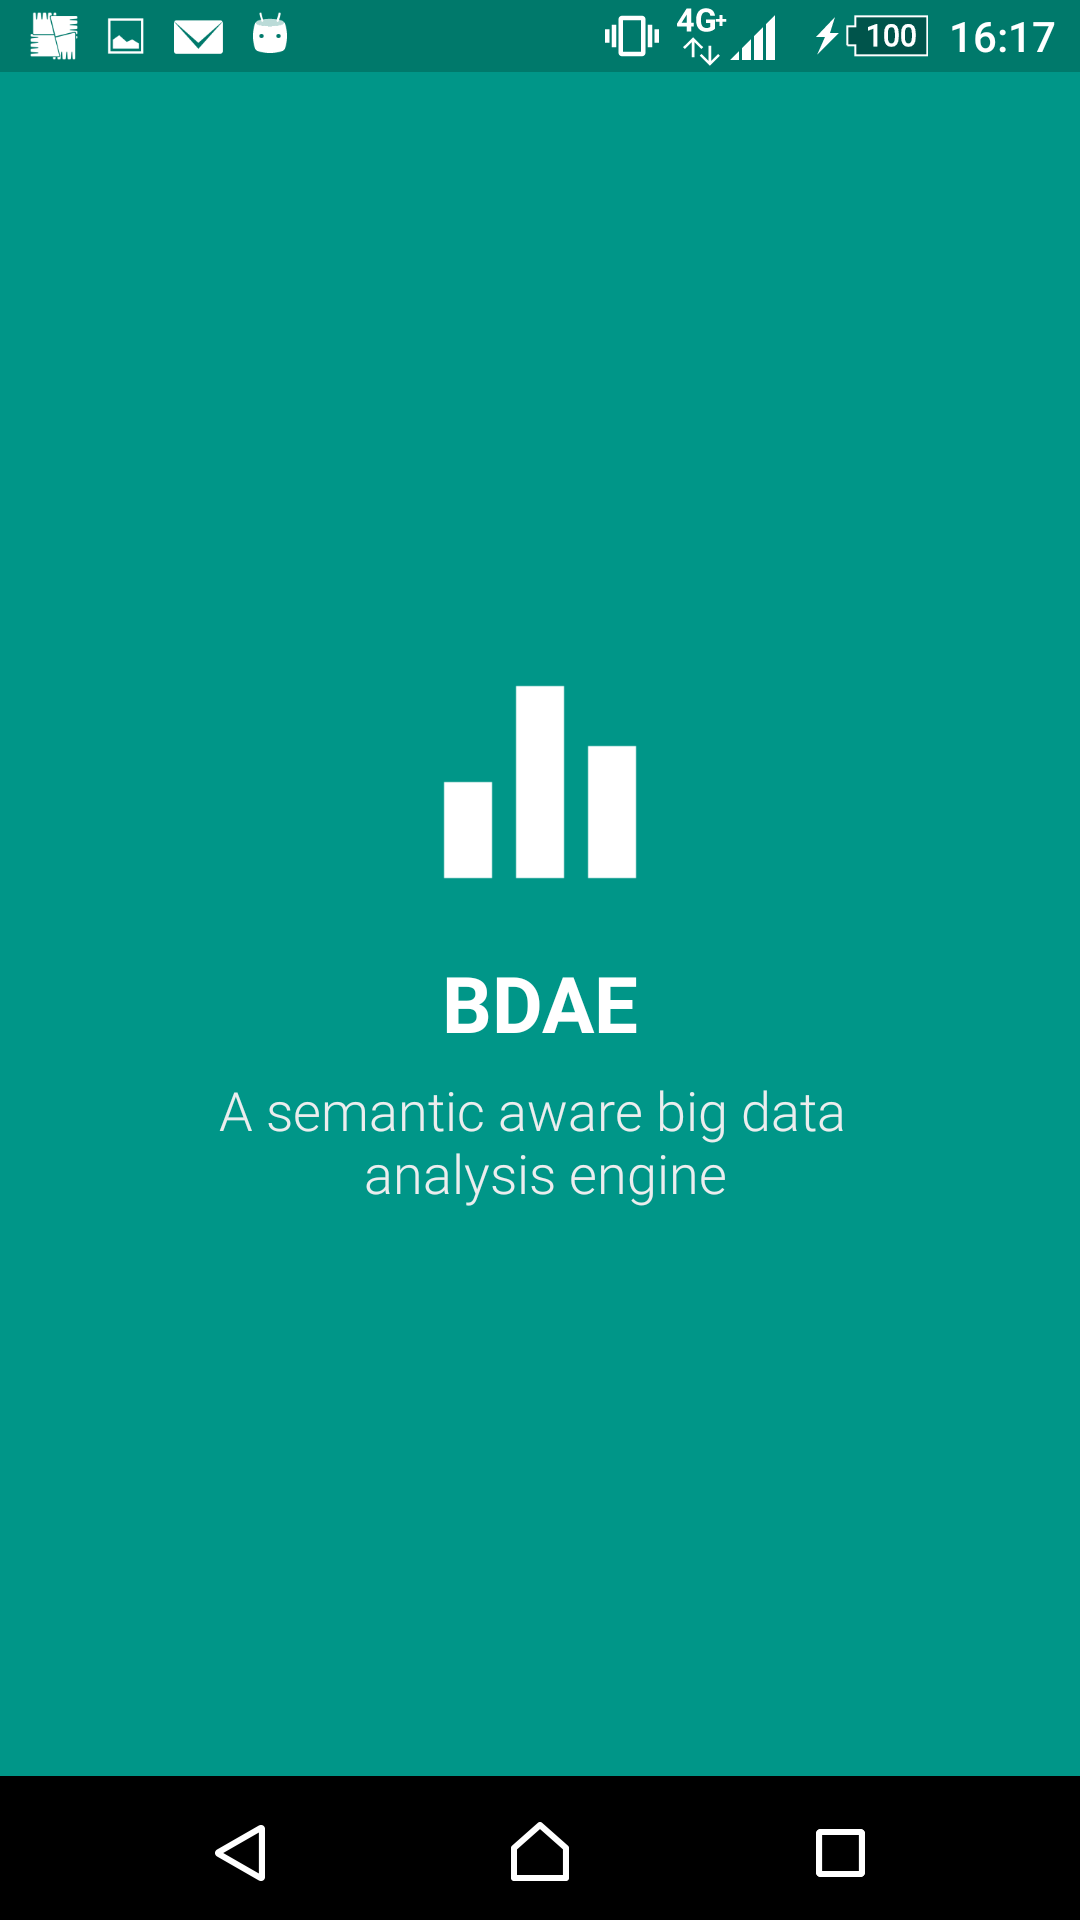
\includegraphics[width=\textwidth]{img/loadingscreen.png}
    \end{minipage}
  	\hfill
  	\begin{minipage}[b]{0.4\textwidth}
    		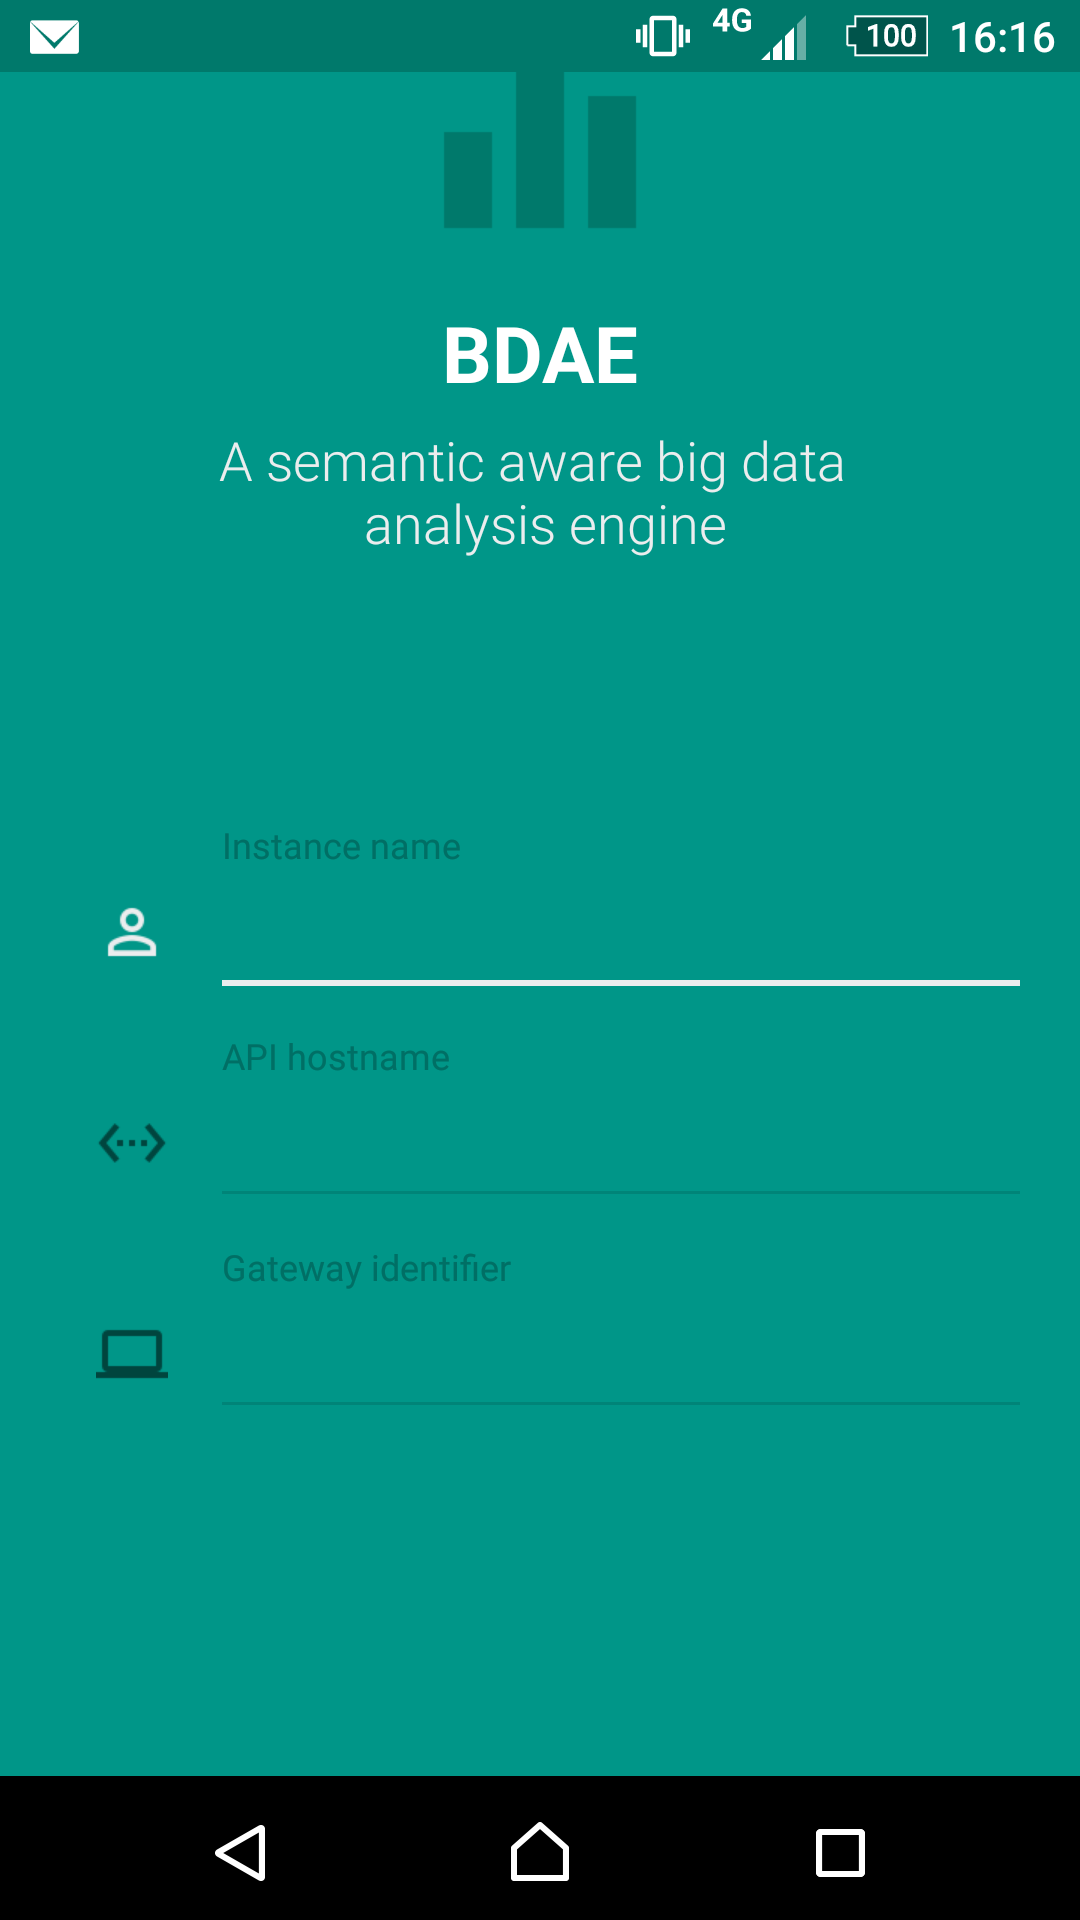
\includegraphics[width=\textwidth]{img/information.png}
  	\end{minipage}
  	\caption[]{Loading screen animated into the required information screen.}
\end{figure*}

\begin{figure*}[h!]
	\centering
  	\begin{minipage}[b]{0.4\textwidth}
    		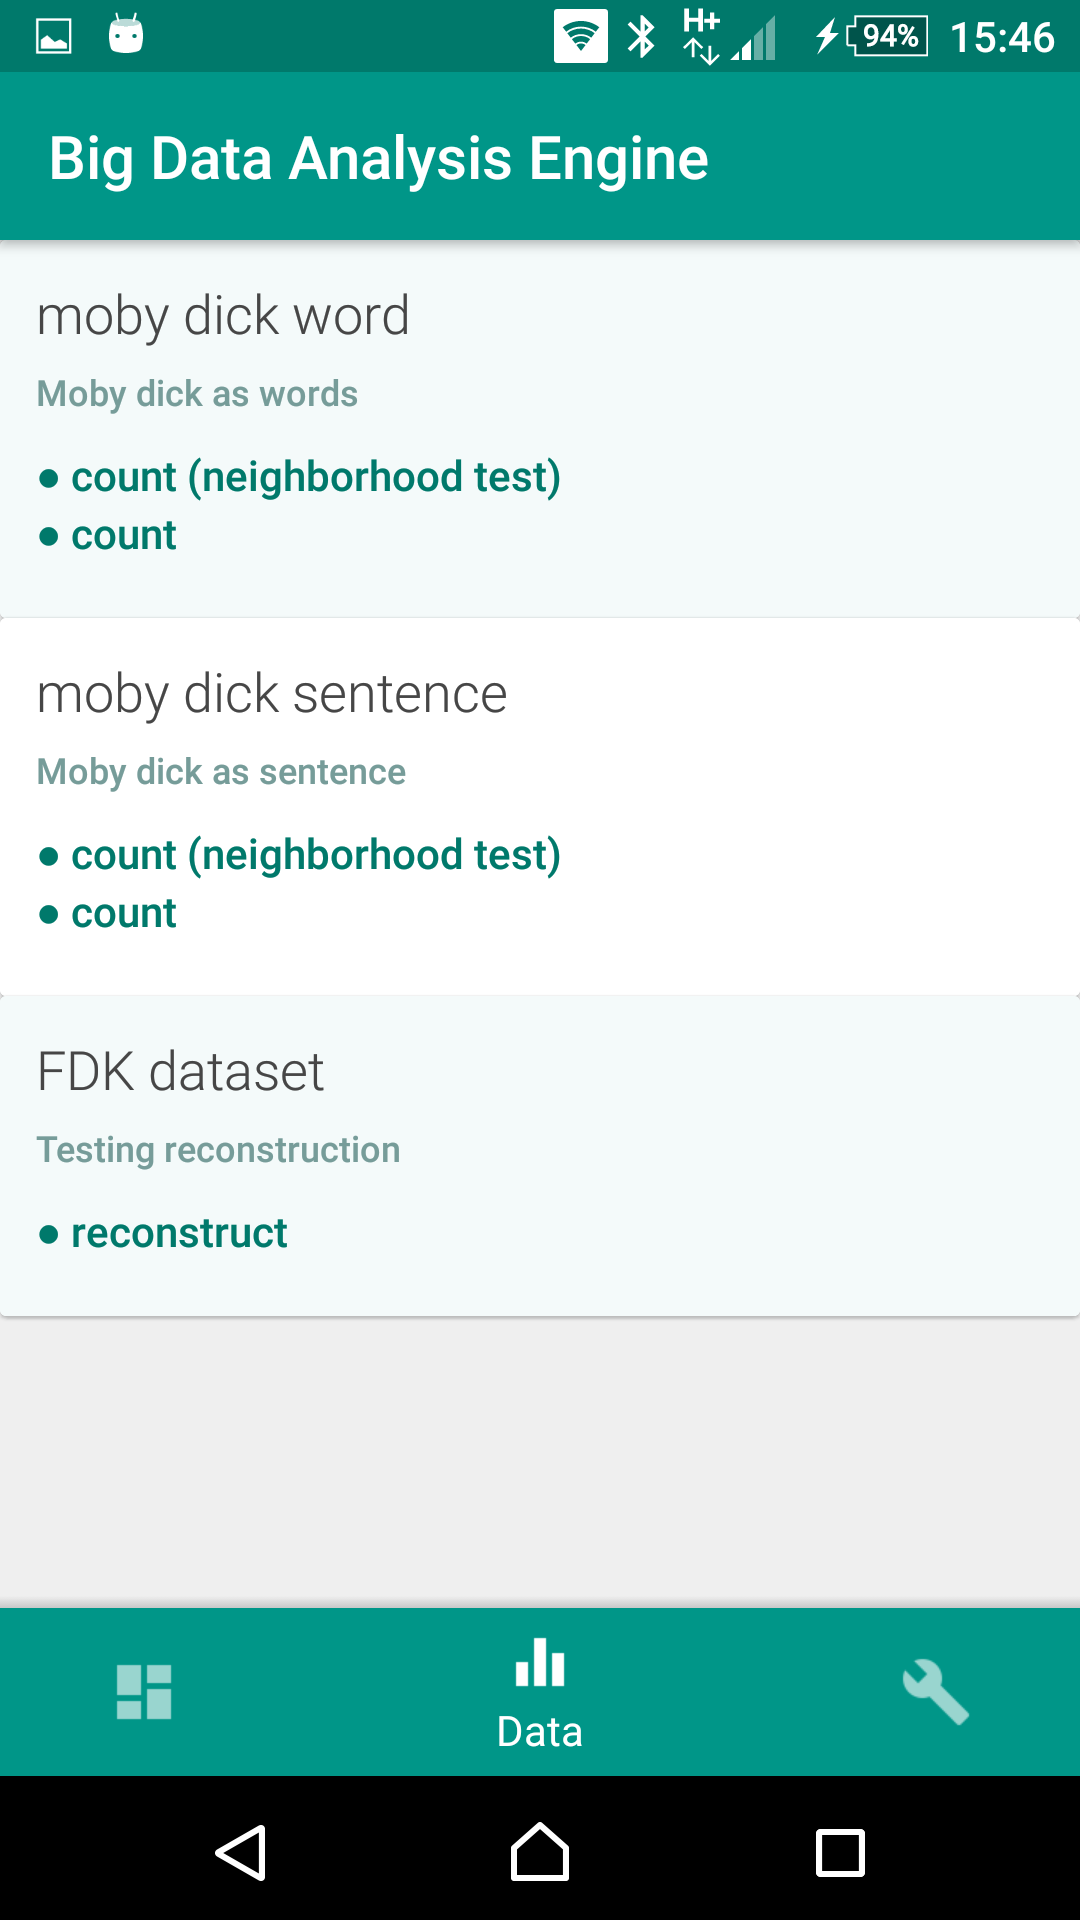
\includegraphics[width=\textwidth]{img/datasets.png}
   	  	\caption[]{List of available datasets and their associated operations.}
    \end{minipage}
  	\hfill
  	\begin{minipage}[b]{0.4\textwidth}
    		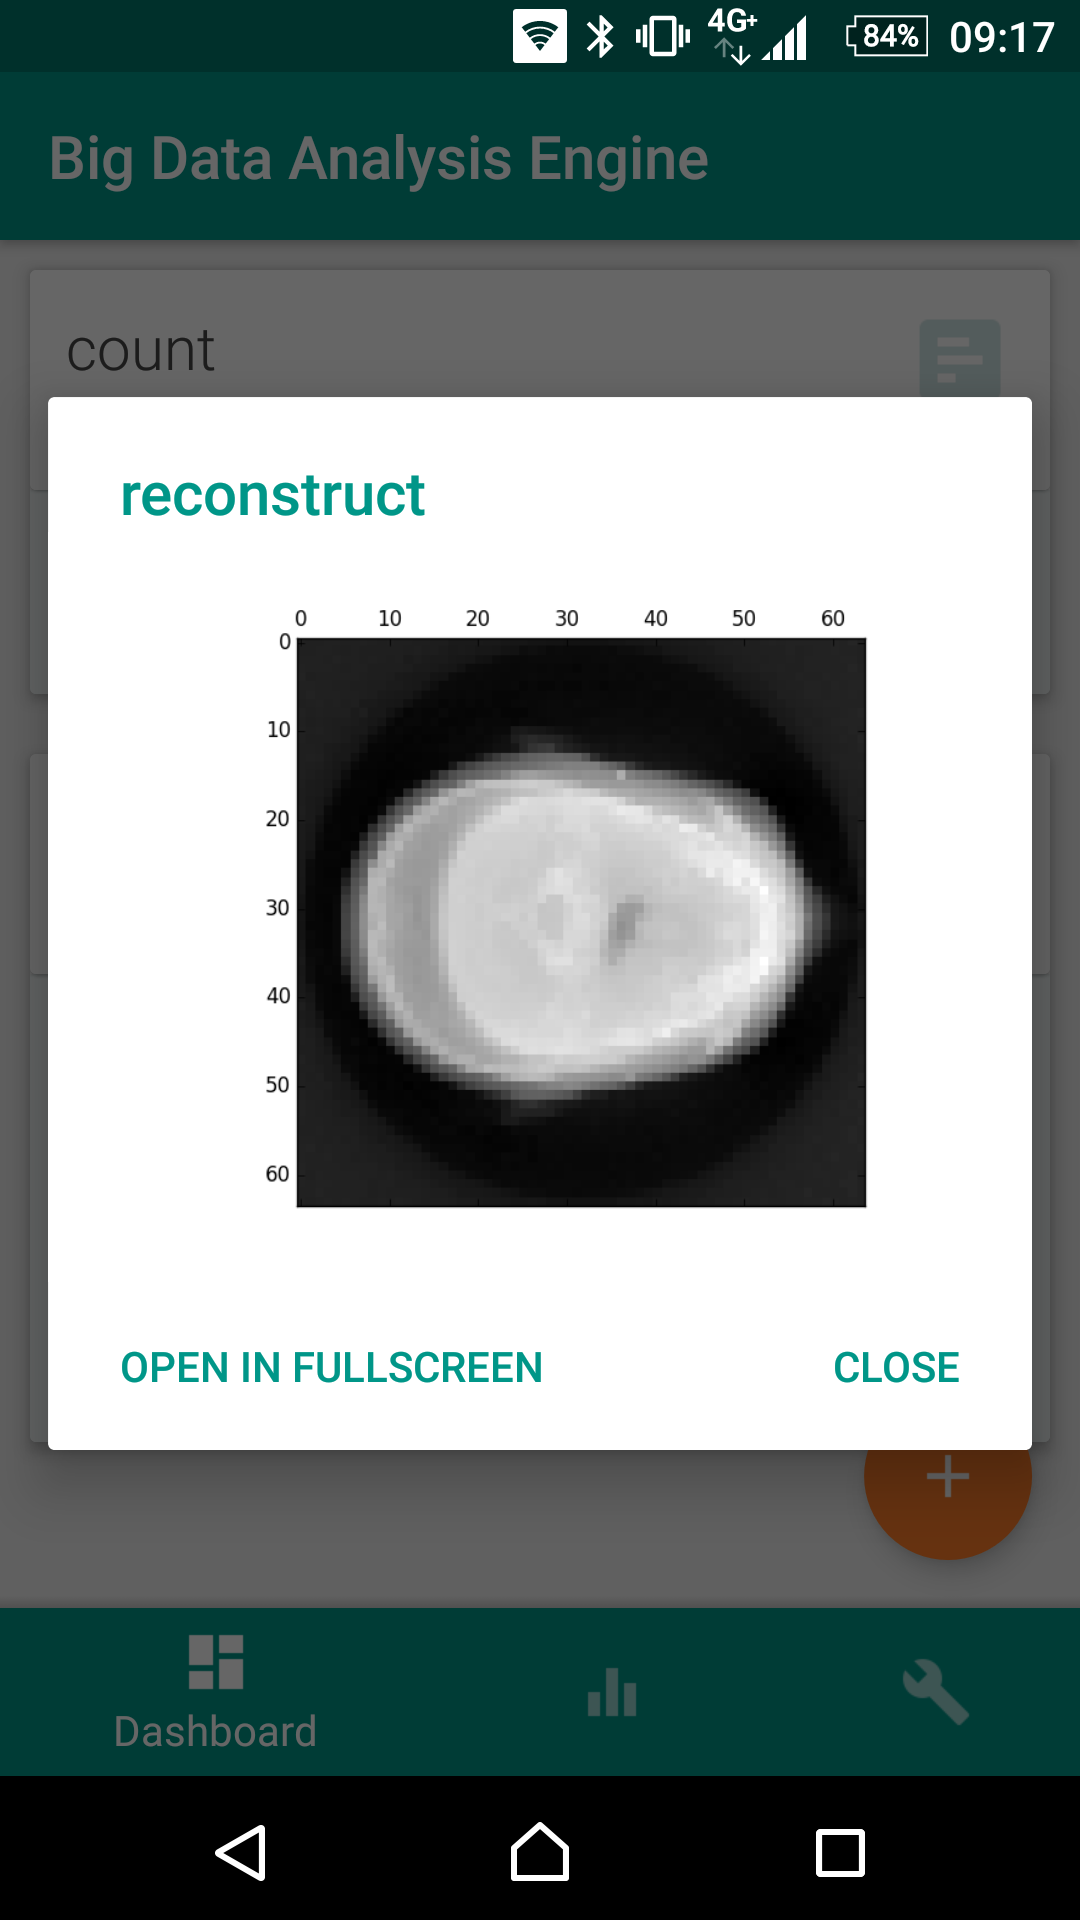
\includegraphics[width=\textwidth]{img/result.png}
    		\caption[]{A dialog displaying the result of a CT reconstruction operation.}
  	\end{minipage}
\end{figure*}